\section[Анализ предметной области]{АНАЛИЗ ПРЕДМЕТНОЙ ОБЛАСТИ}

\subsection{Понятие избыточности данных}

\textit{Избыточность данных} --- центральное понятие в теории сжатия информации.
Простейшим примером избыточности является повторение в тексте одинаковых
фрагментов (например, слов естественного или машинного языка).
Другой вид избыточности заключается в том,
что некоторые фрагменты в сжимаемых данных встречаются чаще других.

Сжатие данных достигается сокращением и удалением из них
избыточности.

Нетрудно показать, что не существует алгоритма, который бы позволял
эффективно сжимать любые файлы.
Любой метод может эффективно сжимать лишь малую долю файлов,
которые не являются случайными. 
Подавляющее число случайных или близких к
случайным файлов не поддается сжатию~\cite{salmon2004}. 
К счастью, именно неслучайные файлы,
представляющие для нас практический интерес,
обладают избыточностью, а, следовательно, могут быть сжаты.

\subsection{Классификация методов сжатия данных}

Методы сжатия данных можно различать по различным признакам.
Рассмотрим некоторые из них.

Во-первых, методы сжатия данных можно классифицировать 
по наличию потерь при сжатии.

\textit{Сжатие без потерь} основано на устранении избыточности, 
содержащейся в исходных данных. 
Сжатие без потерь обычно используется для передачи и хранения текстовых данных,
компьютерных программ, реже~---~для сокращения объёма аудио- и видеоданных,
цифровых фотографий и т. п., в случаях,
когда искажения недопустимы или нежелательны.

Существует два основных подхода к сжатию данных без потерь:
статистический и словарный. 
\textit{Статистический подход} предполагает сжатие данных
на основании частоты их встречаемости в исходном файле. Более подробно
данный подход рассмотрен в подразделе~\ref{ssec:statistical_methods}.
\textit{Словарный подход} предполагает замену часто повторяющихся фрагментов
исходного файла ссылками на словарь, прикрепляемый к сжатой версии. 

\textit{Сжатие данных с потерями} используется в тех случаях,
когда данные не обладают свойством избыточности. Его использование
приемлемо в тех случаях, когда точное совпадение оригинального и сжатого
варианта данных не требуются.
Сжатие с потерями обычно применяется для сокращения объёма аудио- и видеоданных
и цифровых фотографий в тех случаях, когда такое сокращение является
приоритетным, а полное соответствие исходных и восстановленных данных
не требуется.

Во-вторых, методы сжатия данных можно классифицировать 
по виду модели избыточности.

\textit{Модель избыточности} --- набор априорных сведений о характере
избыточноти данных. Иными словами, это информация о том, какие данные
подвергаются сжатию. Не обладая подобной информацией, 
невозможно сделать никаких предположений о преобразовании, 
которое позволило бы уменьшить объём данных.

\textit{Неадаптивная модель избыточности} подразумевает неспособность 
алгоритма сжатия данных изменять свои параметры в зависимости 
от сжимаемых данных. Использование такой модели оправданно 
при для сжатия однотипных данных заранее известного вида, 
например, факсимильных сообщений.

\textit{Адаптивная модель избыточности} предполагает предварительное 
исследование сжимаемых данных с последующей подстройкой параметров алгоритма.

Наконец, методы сжатия данных можно классифицировать 
по уровню производительности.

\textit{Коэффициент сжатия} представляет собой отношение объемов
занимамого пространства исходных и сжатых данных.
Например, коэффициент 0{,}6 означает, что сжатые данные занимают
60\% от исходного размера. Значения, большие одного говорят о том,
что выходной файл больше входного (отрицательное сжатие).
Коэффициент сжатия принято измерять в bpb (bit per bit, бит на бит),
так как он показывает, сколько в среднем понадобится бит сжатого файла
для представления одного бита файла на входе. 

\newpage

\subsection{Статистические методы сжатия данных без потерь}
\label{ssec:statistical_methods}

Статистические методы компрессии используют статистические свойства
сжимаемых данных и присваивают всем символам коды с переменной длиной.
Под <<статистическими свойствами>> обычно понимается вероятность 
(или, что то же самое, частота появления) каждого символа в потоке данных,
однако этот термин может иметь иное, более сложное значение.

Полученные данные используются для назначения более коротких кодов 
более часто встречающимся символам, а более длинных --- редко встречающимся.

Кроме этого, назначаемые коды должны удовлетвоярть \textit{свойству префиксности}:
если некоторая последовательность битов выбрана в качестве кода
какого-то символа, то ни один код другого символа не должен иметь
в начале эту последовательность (не может быть префиксом).
Это требование требуется для однозначного декодирования сжатых данных.

Далее в данной работе будет рассматриваться простой статистический
алгоритм сжатия данных без потерь --- кодирование Хаффмана.

\subsection{Кодирование Хаффмана}
\label{ssec:huffman_encode}

Кодирование Хаффмана является простым алгоритмом для построения
кодов переменной длины, имеющих минимальную среднюю длину.
Этот весьма популярный алгоритм служит основой многих компьютерных программ
сжатия текстовой и графической информации.

Алгоритм начинается составлением списка символов алфавита в
порядке убывания их вероятностей. Затем от корня строится дерево,
листьями которого служат эти символы. Это делается по шагам,
причем на каждом шаге выбираются два символа с наименьшими
вероятностями, добавляются наверх частичного дерева, удаляются
из списка и заменяются вспомогательным символом, представляющим
эти два символа. Вспомогательному символу приписывается
вероятность, равная сумме вероятностей, выбранных на этом 
шаге символов. Когда список сокращается до одного вспомогательного символа,
представляющего весь алфавит, дерево объявляется
построенным.
Завершается алгоритм спуском по дереву и построением кодов всех символов.

Вероятности и частоты следует записать в сжатый файл для того,
чтобы декомпрессор (декодер) Хаффмана мог сделать декомпрессию данных.
На рисунке~\ref{pic:huffman_en} приведен код Хаффмана для английского алфавита.

\begin{figure}[h]
  \centering
  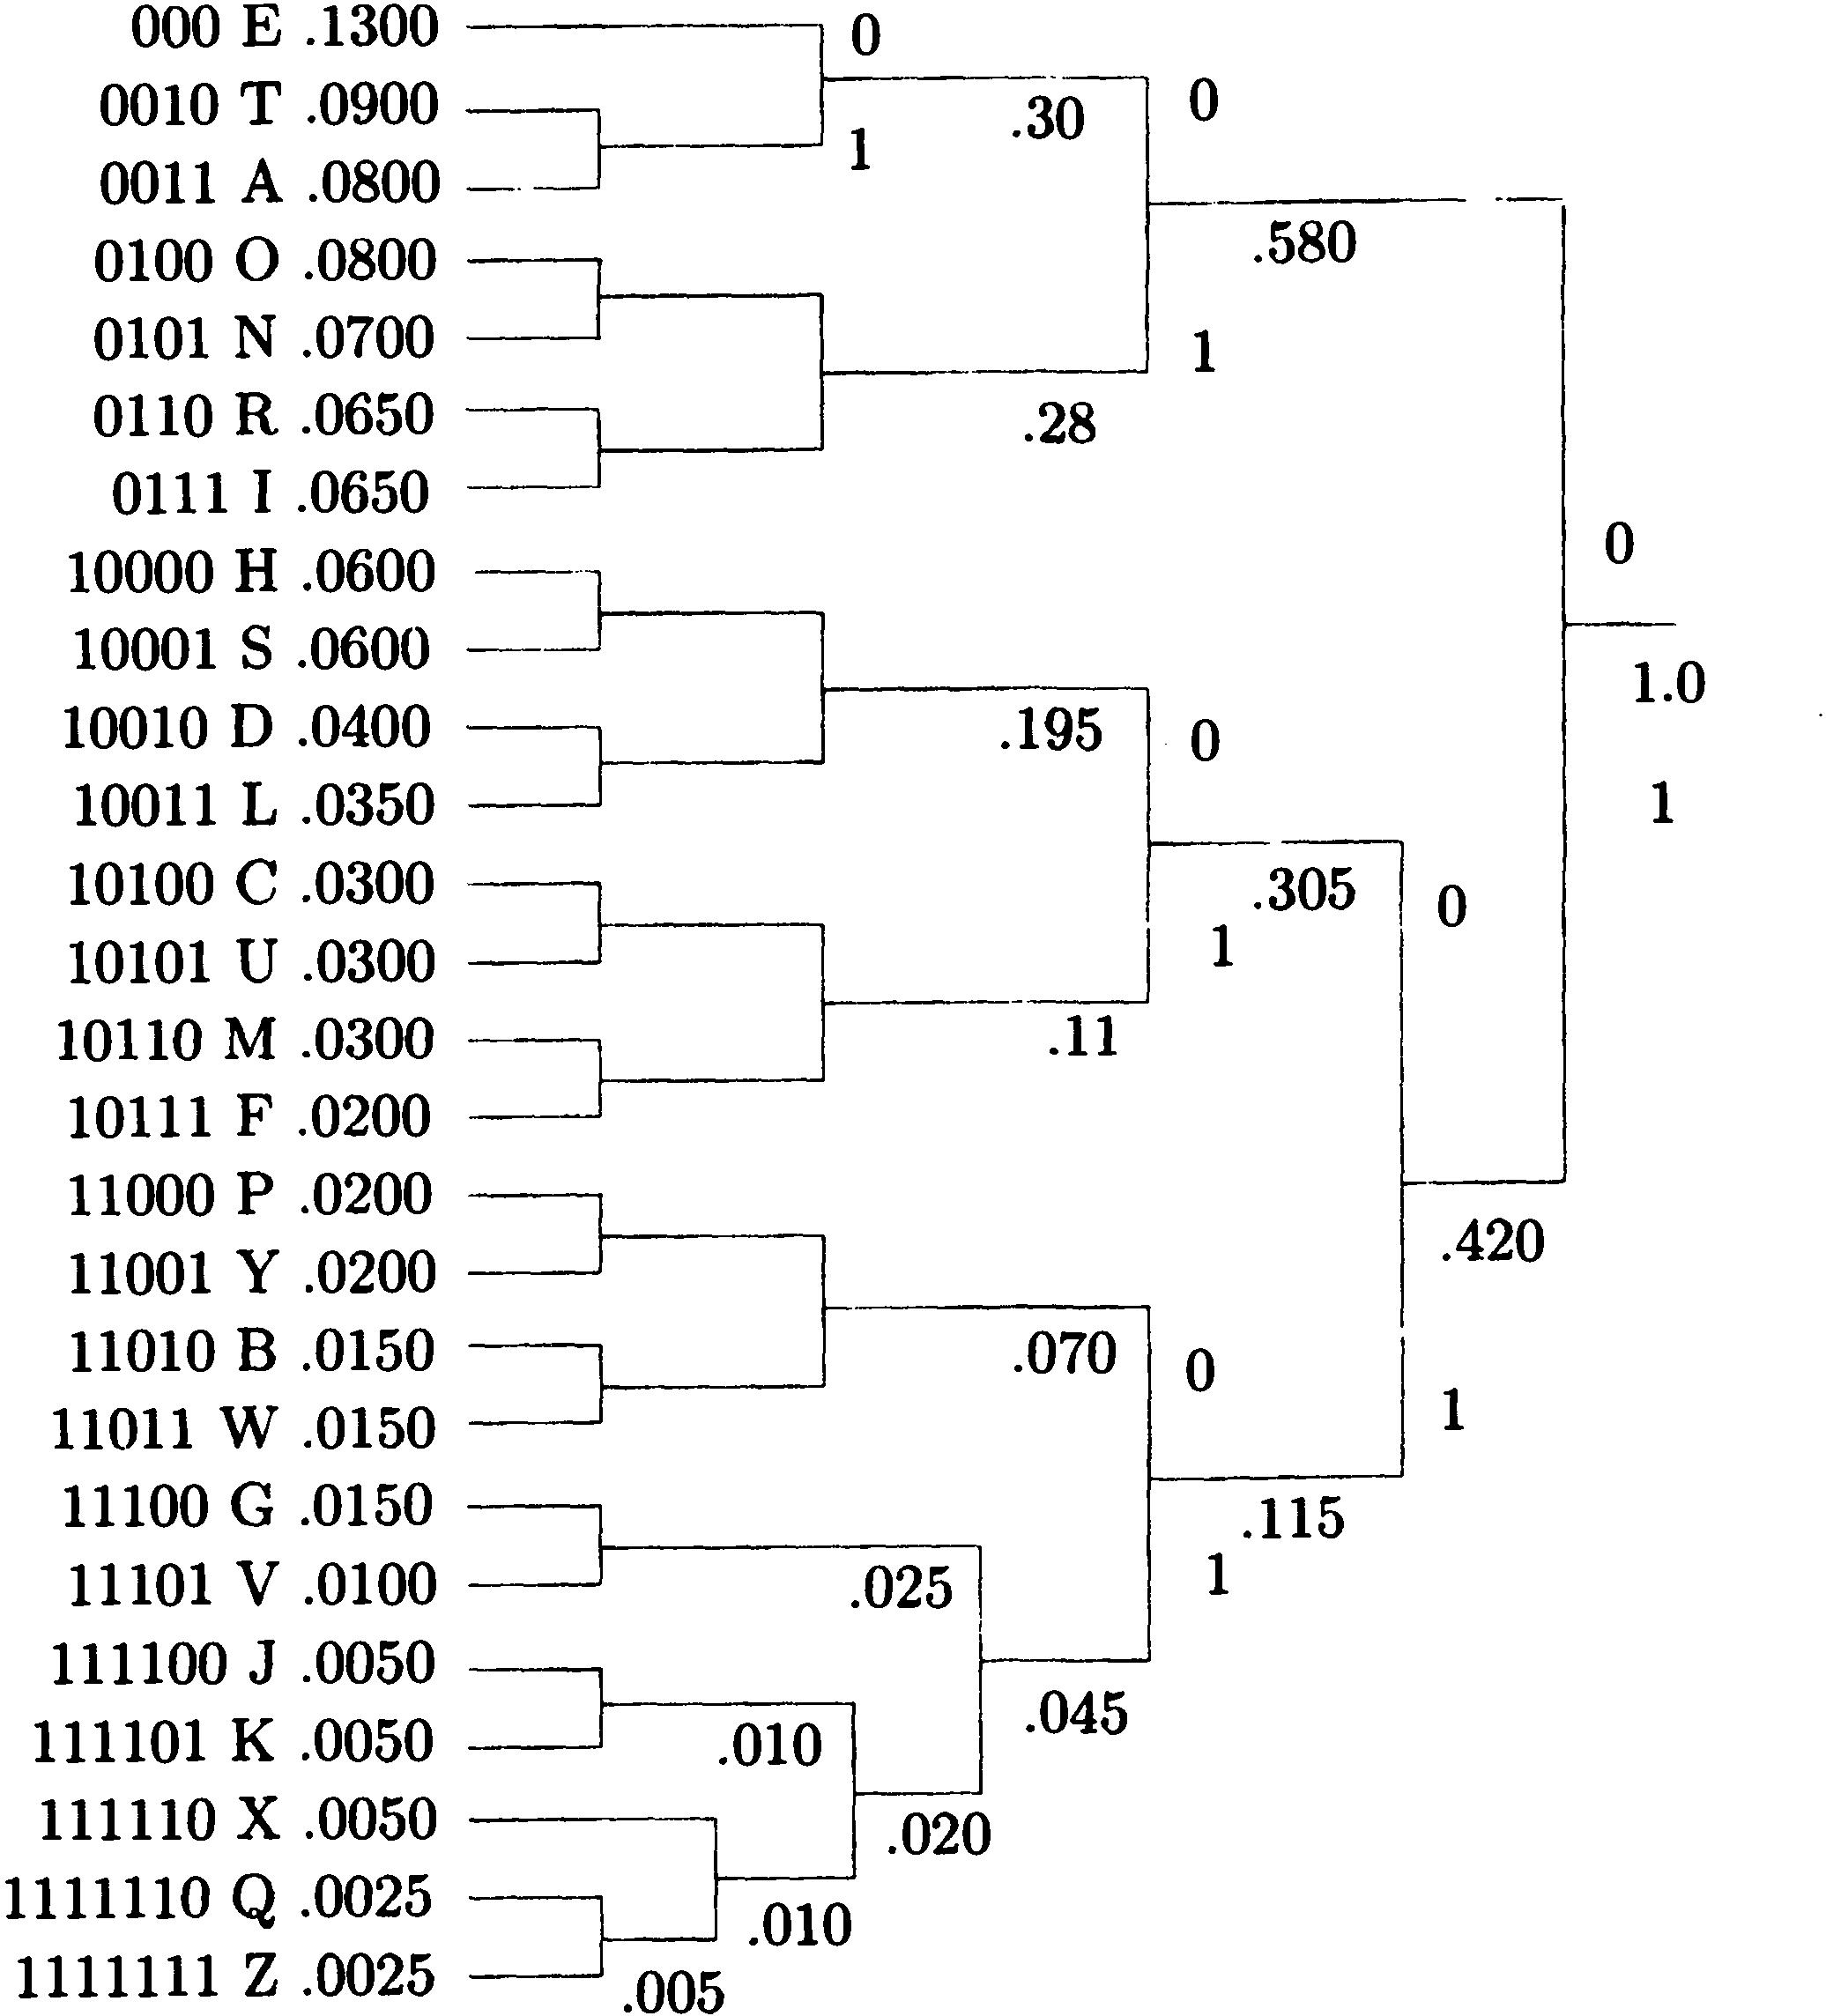
\includegraphics[width=150mm]{pic/huffman_en.jpg}
  \caption{Код Хаффмана для английского алфавита}
  \label{pic:huffman_en}
\end{figure}

Из этого рисунка видно, что символам с большей вероятностью соответствуют
коды меньшей длины. Доказано, что сжатие с использованием кодов Хаффмана
является наиболее эффективным в тех случаях, когда вероятности вхождения символов
в файл-источник равны $ 2^{-n}, n=1,2,3,\dots $ 

\subsection{Декодирование Хаффмана}
\label{ssec:huffman_decode}

Перед началом декодирования, декодер должен прочесть начало 
файла и построить дерево Хаффмана для алфавита.
Только после этого он может читать и декодировать весь файл.
Алгоритм декодирования очень прост.
Следует начать с корня и прочитать первый бит сжатого файла.
Если это нуль, следует двигаться по нижней ветке дерева;
если это единица, то двигаться надо по верхней ветке дерева.
Далее читается второй бит и происходит движение по следующей
ветке по направлению к листьям. Когда декодер достигнет листа
дерева, он узнает код первого несжатого символа 
(обычно это символ ASCII).
Процедура повторяется для следующего бита, начиная опять из корня дерева.

Описанная процедура проиллюстрирована на рисунке~\ref{pic:huffman_de}
для алфавита из пяти символов. 

\begin{figure}[h]
  \centering
  {
    % \vspace{7pt}
    \setlength{\fboxsep}{0pt}%
    \setlength{\fboxrule}{1pt}%
    \fbox{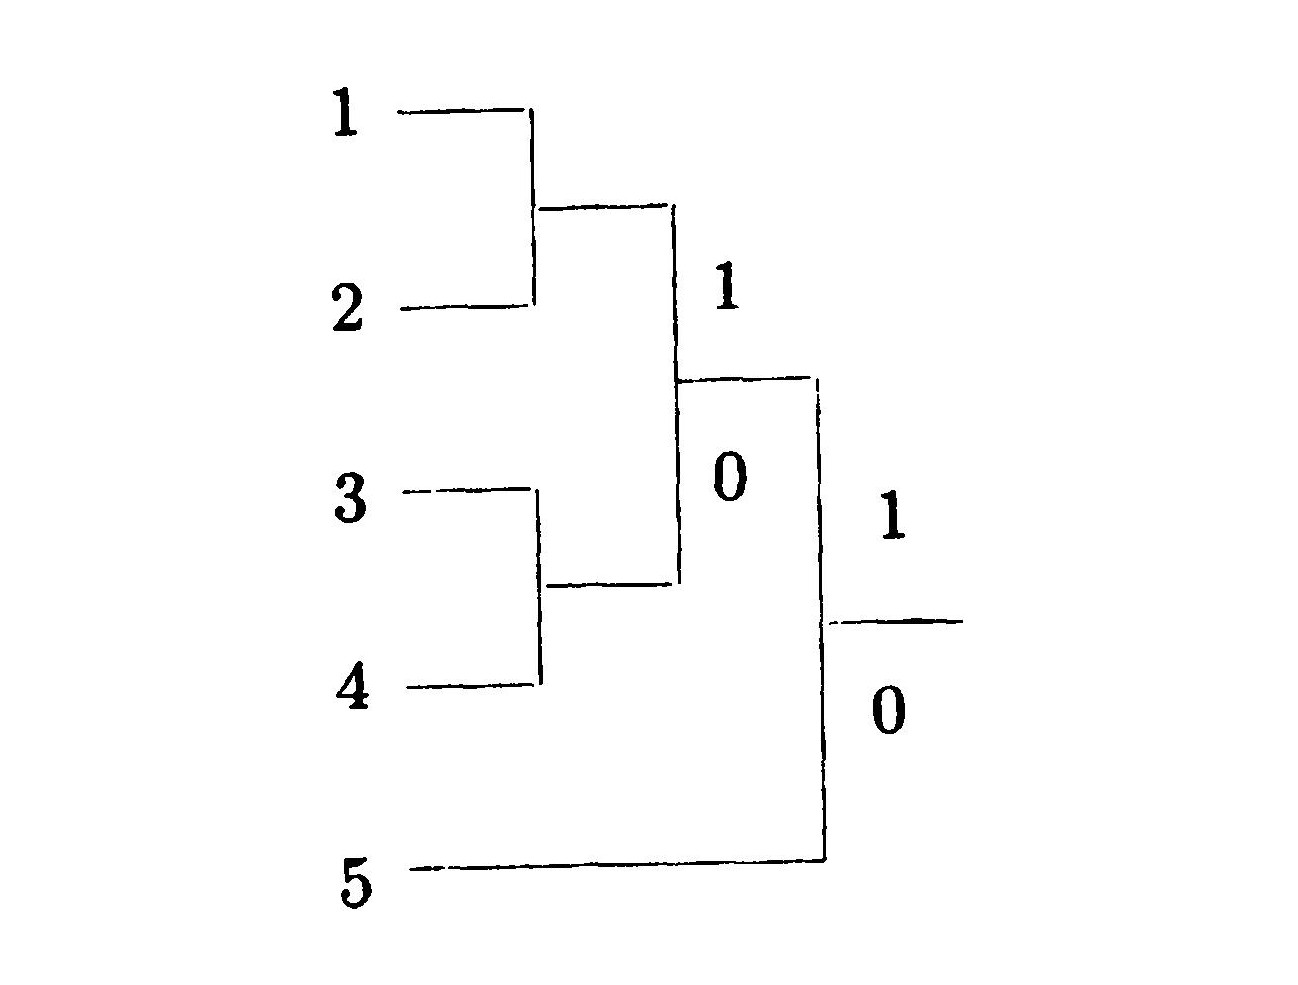
\includegraphics[width=100mm]{pic/huffman_de.jpg}}
    % \vspace{7pt}
  }
  \caption{Декодирование Хаффмана}
  \label{pic:huffman_de}
\end{figure}

Входная строка $a_4a_2a_5a_1$ кодируется
последовательностью 1001100111. Декодер начинает с корня, читает первый
бит <<1>> и идет вверх. Второй бит <<0>> направляет его вниз. 
То же самое делает третий бит. Это приводит декодер к листу $a_4$.
Получен первый несжатый символ. Декодер возвращается в корень и читает
110, движется вверх, вверх и вниз и получает символ $a_2$, и так далее.

\subsection{Постановка задачи}

Требуется разработать консольное приложение, способное
выполнять сжатие и расжатие данных с помощью алгоритма Хаффмана.

Данное приложение должно иметь высокую производительность при 
низких системных требованиях
(X86-совместимый компьютер с тактовой
частотой процессора 500 МГц,
объемом оперативной памяти 64~МБ) 
и работать под управлением различных операционных систем
(ОС на базе ядра GNU/Linux, *BSD, Windows).

